\documentclass[draft]{article}
\usepackage{cmap}
\usepackage[T1,T2A]{fontenc}
\usepackage[utf8]{inputenc}
\usepackage[russian]{babel}
\usepackage[left=2cm,right=2cm,top=2cm,bottom=2cm,bindingoffset=0cm]{geometry}
\usepackage{tikz}


\usepackage{setspace,amsmath}
\usepackage{lipsum}
\usepackage[usestackEOL]{stackengine}
\usepackage{kantlipsum}
\usepackage{graphicx}
\usepackage{caption}
\usepackage{float}
\usetikzlibrary{positioning}
\graphicspath{{pictures/}}
\DeclareGraphicsExtensions{.pdf,.png,.jpg}
\newcommand\zz[1]{\par{\normalsize\strut #1} \hfill\ignorespaces}
\addto\captionsrussian{\def\refname{List of used sources}}
\newcommand{\subtitle}[1]{%
  \posttitle{%
    \par\end{center}
    \begin{center}\Large#1\end{center}
   }%
}
\newcommand{\subsubtitle}[1]{%
  \preauthor{%
    \begin{center}
    \large #1 \vskip0.5em
    \begin{tabular}[t]{c}
    }%
}
\newcommand\tab[1][1cm]{\hspace*{#1}}
\begin{document}
 
\begin{center}
\textbf{
ПРАВИТЕЛЬСТВО РОССИЙСКОЙ ФЕДЕРАЦИИ\\
НАЦИОНАЛЬНЫЙ ИССЛЕДОВАТЕЛЬСКИЙ УНИВЕРСИТЕТ\\
«ВЫСШАЯ ШКОЛА ЭКОНОМИКИ»\\
Факультет компьютерных наук
Образовательная программа «Программная инженерия»\\
(ВШЭ ФКН ПИ)}\\
\end{center}
УДК 004.852
\bigskip
\zz{СОГЛАСОВАНО}УТВЕРЖДАЮ
\zz{Руководитель,}Академический руководитель
\zz{Стажер-исследователь,}образовательной программы
\zz{приглашённый лектор}«Программная инженерия»
\zz{\noindent\rule{3cm}{0.4pt} О. Н. Качан}профессор департамента программной
\zz{«\noindent\rule{1cm}{0.4pt}»\noindent\rule{2cm}{0.4pt}20\noindent\rule{0.5cm}{0.4pt}г.}инженерии, канд. техн. наук
\zz{~}\noindent\rule{3cm}{0.4pt} В.В. Шилов
\zz{~}«\noindent\rule{1cm}{0.4pt}»\noindent\rule{2cm}{0.4pt}20\noindent\rule{0.5cm}{0.4pt}г.
\begin{center}
\topskip=0pt
\vspace*{\fill}
\textbf{ОТЧЕТ\\
О НАУЧНО-ИССЛЕДОВАТЕЛЬСКОЙ РАБОТЕ}\\
~\\
SYNCHRONIZATION OF NEUROMORPHIC NETWORKS OF THE CLOSE WORLD FROM THE POINT OF VIEW OF COMPLEXES\\
(заключительный)\\
\vspace*{\fill}
\end{center}
\zz{~}Выполнил:
\zz{~}Студент группы БПИ204
\zz{~}образовательной программы
\zz{~}«Программная инженерия»
\zz{~}Пеганов Никита Сергеевич
\zz{~}\noindent\rule{3cm}{0.4pt} Н. С. Пеганов
\zz{~}«\noindent\rule{1cm}{0.4pt}»\noindent\rule{2cm}{0.4pt}20\noindent\rule{0.5cm}{0.4pt}г.
\begin{center}
\vspace*{\fill}{
  Москва 2022}
\end{center}
\newpage
\begin{center}
\section {Abstract}
\end{center}

\newpage
\begin{center}
\section {Content}
\tableofcontents
\end{center}
\newpage
\section {Basic terms, definitions and abbreviations}
\textbf{Graph} — a set of items connected by edges. A graph G can be defined as a pair (V,E), where V is a set of vertices, and E is a set of edges between the vertices  $E \subseteq \{(u,v) | u, v \in V\}$\cite{litlink1}.\\
\textbf{Simplicial complex} $K$ (sometimes called an abstract simplicial complex) consists of
\begin{enumerate} 
\item a set of objects, V(K), called vertices
\item a set, $S(K)$, of finite non-empty subsets of $V(K)$, called simplices.
\end{enumerate}
such that the simplices satisfy the following conditions:
\begin{enumerate} 
\item if $\sigma\subset V(K)$ is a simplex and $\tau\subset\sigma, \tau\neq\emptyset$, then $\tau$ is also a simplex;
\item every singleton {v}, $v\in V(K)$, is a simplex\cite{litlink4}.
\end{enumerate}
\textbf{Dynamical systems on graphs and complexes}\\
\textbf{Synchronization} — the fact of happening at the same time, or the act of making things happen at the same time\cite{litlink2}.\\
\textbf{Simplicial synchronization} — a fundamental dynamical state observed in a wide variety of complex systems and capturing among other phenomena important aspects of brain dynamics and circadian rhythms\cite{litlink3}.\\
\textbf{Kuramoto model} is a stylized model that explains how coupled oscillators, that in absence of interactions would have different intrinsic frequencies, can start to follow a collective coherent motion when their coupling constant $\sigma$, measuring the strength of their interaction, is larger than a critical value $\sigma_c$ also called synchronization threshold\cite{litlink3}.\\
\newpage
\begin{center}
\item\section {Introduction}
\end{center}
\textbf{Task description}\\
~\\
\textbf{Relevance}\\
~\\
\textbf{Subject of research}\\
~\\
\textbf{Research methods}\\
~\\
\textbf{Purposes and objectives of the work}\\
~\\
\textbf{Originality and reliability of the obtained results}\\
~\\
\textbf{Theoretical significance}\\
~\\
\textbf{Practical value}\\
~\\
\newpage
\begin{center}
\section {The main part of the research report}
\end{center}
\textbf{Review and analysis of sources}\\
\tab\textbf{"Geometry, Topology and Simplicial Synchronization"\cite{litlink3}} by Ana Paula Millán, Juan G. Restrepo, Joaquín J. Torres and Ginestra Bianconi is a review article fully covering the area under study. It defines "Simplicial synchronization", "Kuramoto model", "Graph Laplacian" and other important definitions. \\
\tab In this article Ginestra Bianconi explores how the combinatorial and statistical properties of complex networks have effects on dynamics. Simplical complexes affect on higher-order dynamics through simplical geometry and topology. To research it two frameworks are used: Network Geometry with Flavor (NGF) and Graph Laplacian. Exactly, spectral dimension of NGF networks is used to measure the gemetry influence on dynamics.\\
\tab The level of synchronization in the system is measured by the
Kuramoto order parameter,
\begin{center}
$Z_0 = R_0e^{i\Theta} = \frac{1}{N} \sum_{j=1}^{N_[0]}e^{i\theta _j}$,
\end{center}
where $R_0$ and $\Theta$ are both real and where $0<=R_0<=1$ measures the overall coherence and $\Theta = \Theta (t)$ is the phase of global oscillations.
\tab As the result of the research we have several formulas that can determine the level of syncronization of complexes with differtent geometry and topology.
\begin{figure}[h]
\center{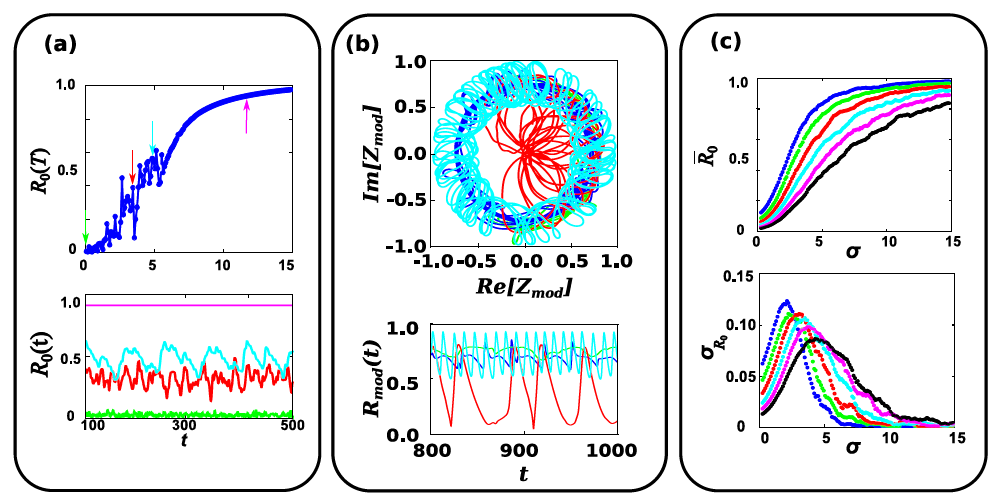
\includegraphics[draft=false,width=1\linewidth]{Fig1}}
\caption{Frustrated synchronization on NGF characterized by spatio-temporal fluctuations of the order parameter\cite{litlink3}.}
\label{ris:image}
\end{figure}\\
\tab \textbf{"Higher-order simplicial synchronization of coupled topological signals"\cite{litlink5}} by Reza Ghorbanchian, Juan G. Restrepo, Joaquin J. Torresy, and Ginestra Bianconi shows the possible phase transitions that can occur when topological signals dened on nodes and links interact. This research is based on the mathematical framework of higher-order topological synchronization. For some reasons, in this work authours focus in particular on the coupled synchronization of topological signals dened on nodes and links.\\
\tab Interestingly, in this research more mathematical frameworks has been chosen: models NL and NLT, Geometry with Flavor (NGF) and Kuramoto model for measuring the level of synchronization in the system.\\
\tab This work uncovers how topological signals associated to nodes and links can be coupled to one another giving rise to an explosive synchronization phenomenon involving both signals at the same time. Created model has been tested on real connectomes and on major examples of simplicial complexes (the conguration model of simplicial complex and the Network Geometry with Flavor).\\
~\\
\begin{figure}[h]
\center{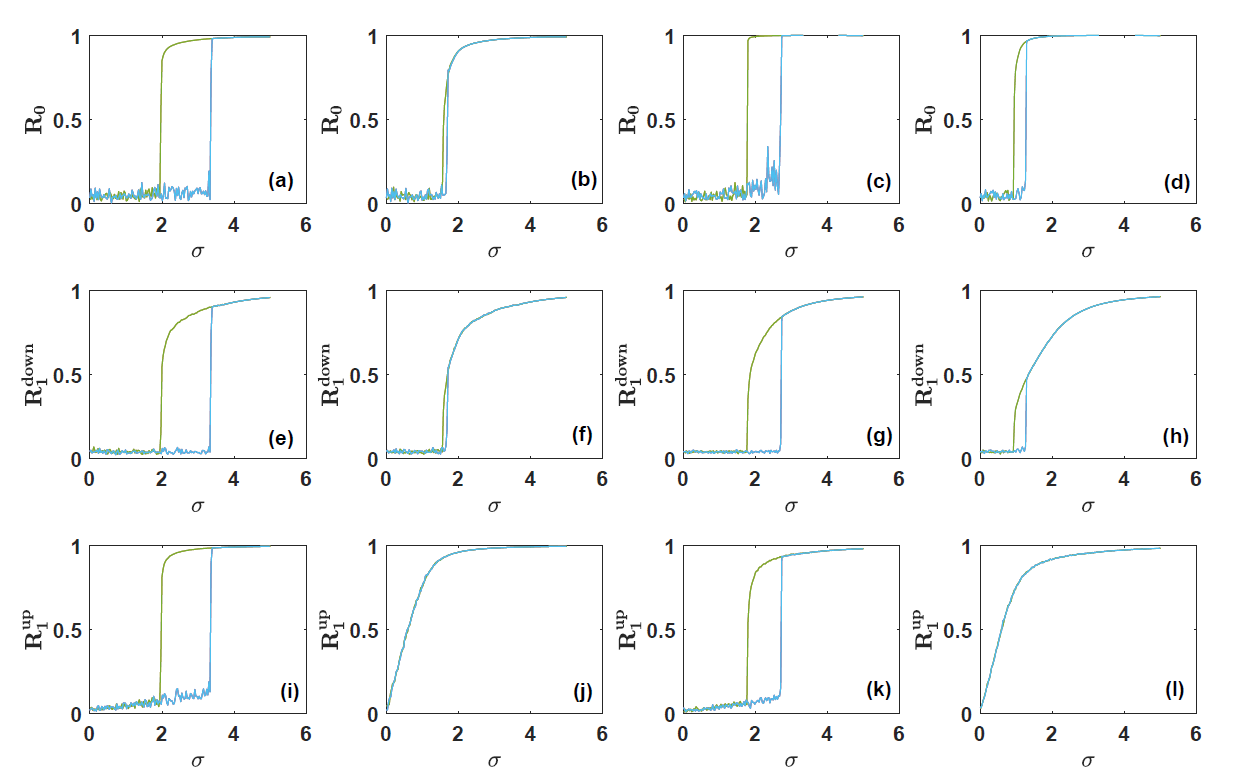
\includegraphics[draft=false,width=1\linewidth]{Fig2}}
\caption{The Higher-order topological synchronization models (Models NL and NLT) coupling nodes and links on simplicial complexes\cite{litlink6}.}
\label{ris:image}
\end{figure}\\
~\\
\tab In work \textbf{"Explosive higher-order Kuramoto dynamics on simplicial complexes"} Ana P. Millán, Joaquín J. Torres, Ginestra Bianconi show, how complexes behave on higher-order interactions.\\
\tab In this work the configuration model Configuration of simplicial complexes is used, which naturally generalizes the configuration model of networks. There are also exist Farber, Emergent, Hyperbolic and Petri-dynamical models.\\
\tab So, authors show, that higher-order Kuramoto dynamics are defined on faces of dimension $n-1$ and $n+1$, which follow a dynamics of coupled oscillators. This work opens innovative perspectives in characterizing the Kuramoto dynamics on higher dimensional simplices.\\
\begin{figure}[h]
\center{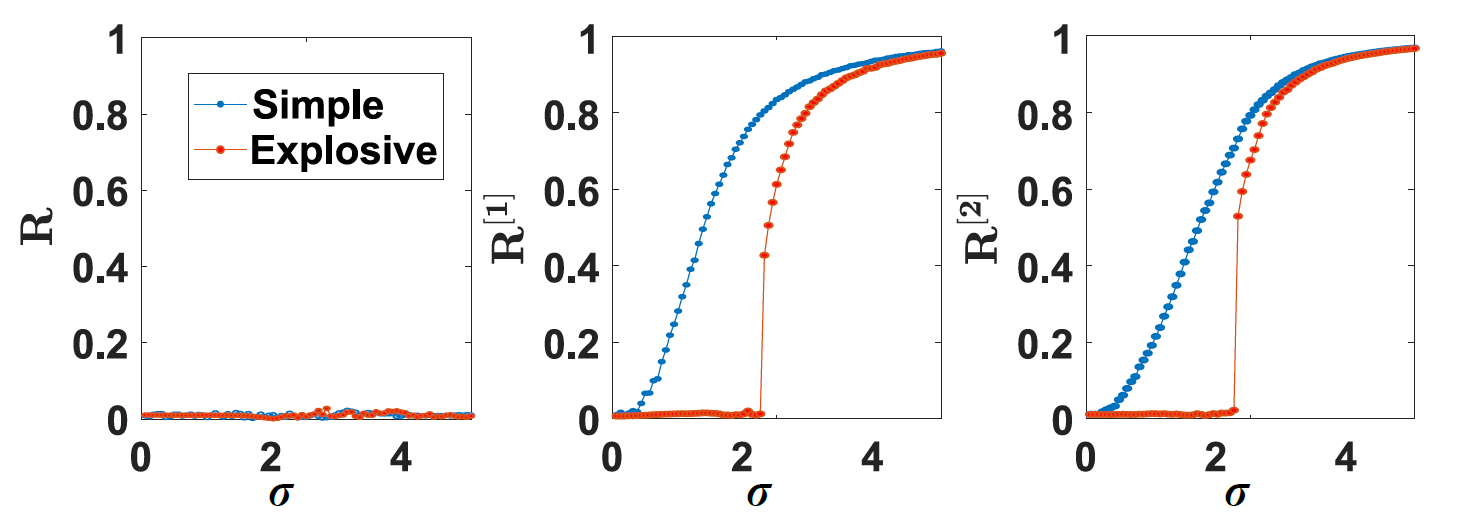
\includegraphics[draft=false,width=1\linewidth/2]{Fig3}}
\caption{The order parameters R, R[1] and R[2] of the simple (blue circles) and explosive (red squares) higher-order $(n = 1)$. Kuramoto dynamics are plotted versus the coupling constant $\sigma$.\cite{litlink7}.}
\label{ris:image}
\end{figure}\\
\textbf{Selection of methods, algorithms, models for solving tasks}\\
~\\
\textbf{Description of selected or proposed methods, algorithms, models, techniques}\\
~\\
\textbf{Description of the experiment}\\
~\\
\textbf{Review and analysis of sources}\\
~\\
\textbf{Description of the experiment}\\
~\\

\newpage
\begin{center}
\section {Conclusion}
\end{center}

\newpage
\begin{center}
\begin{thebibliography}{}
\bibitem{litlink1} \textit{Paul E. Black and Paul J. Tanenbaum} "graph", in Dictionary of Algorithms and Data Structures [online], Paul E. Black, ed. 21 June 2021. (accessed 04.07.2022) Available from: https://www.nist.gov/dads/HTML/graph.html
\bibitem{litlink2} \textit{Cambridge University Press} Meaning of synchronization in English. // Website dictionary.cambridge.org (https://dictionary.cambridge.org/dictionary/english/synchronization). Viewed: 04.07.2022
\bibitem{litlink3} \textit{Ana Paula Millán, Juan G. Restrepo, Joaquín J. Torres and Ginestra Bianconi} Geometry, Topology and Simplicial Synchronization. P. 12
\bibitem{litlink4} Simplicial complex. // Website ncatlab.org (https://ncatlab.org/nlab/show/simplicial+complex). Viewed: 09.07.2022
\bibitem{litlink5} \textit{Reza Ghorbanchian, Juan G. Restrepo, Joaquin J. Torresy, and Ginestra Bianconi} Higher-order simplicial synchronization of coupled topological signals. // Website Arxiv.org (https://arxiv.org/abs/2011.00897). Viewed: 11.07.2022
\bibitem{litlink6} \textit{Reza Ghorbanchian, Juan G. Restrepo, Joaquin J. Torresy, and Ginestra Bianconi} Higher-order simplicial synchronization of coupled topological signals. P. 6
\bibitem{litlink7} \textit{Ana P. Millan, Joaquin J. Torres,  Ginestra Bianconi} Explosive higher-order Kuramoto dynamics on simplicial complexes. // Website Arxiv.org (https://arxiv.org/abs/1912.04405). Viewed: 11.07.2022
\end{thebibliography}
\end{center}
\newpage
\begin{center}
\section {Applications}
\end{center}
\zz{}\textbf{Application 1\\}
Link to the project repository with the source code and all used materials.\\
https://github.com/NikPeg/synchronization-of-neuromorphic-networks-of-the-close-world-from-the-point-of-view-of-complexes\\
\end{document}